%% ut-thesis.tex -- document template for graduate theses at UofT
%%
%% Copyright (c) 1998-2013 Francois Pitt <fpitt@cs.utoronto.ca>
%% last updated at 16:20 (EDT) on Wed 25 Sep 2013
%%
%% This work may be distributed and/or modified under the conditions of
%% the LaTeX Project Public License, either version 1.3c of this license
%% or (at your option) any later version.
%% The latest version of this license is in
%%     http://www.latex-project.org/lppl.txt
%% and version 1.3c or later is part of all distributions of LaTeX
%% version 2005/12/01 or later.
%%
%% This work has the LPPL maintenance status "maintained".
%%
%% The Current Maintainer of this work is
%% Francois Pitt <fpitt@cs.utoronto.ca>.
%%
%% This work consists of the files listed in the accompanying README.

%% SUMMARY OF FEATURES:
%%
%% All environments, commands, and options provided by the `ut-thesis'
%% class will be described below, at the point where they should appear
%% in the document.  See the file `ut-thesis.cls' for more details.
%%
%% To explicitly set the pagestyle of any blank page inserted with
%% \cleardoublepage, use one of \clearemptydoublepage,
%% \clearplaindoublepage, \clearthesisdoublepage, or
%% \clearstandarddoublepage (to use the style currently in effect).
%%
%% For single-spaced quotes or quotations, use the `longquote' and
%% `longquotation' environments.


%%%%%%%%%%%%         PREAMBLE         %%%%%%%%%%%%

%%  - Default settings format a final copy (single-sided, normal
%%    margins, one-and-a-half-spaced with single-spaced notes).
%%  - For a rough copy (double-sided, normal margins, double-spaced,
%%    with the word "DRAFT" printed at each corner of every page), use
%%    the `draft' option.
%%  - The default global line spacing can be changed with one of the
%%    options `singlespaced', `onehalfspaced', or `doublespaced'.
%%  - Footnotes and marginal notes are all single-spaced by default, but
%%    can be made to have the same spacing as the rest of the document
%%    by using the option `standardspacednotes'.
%%  - The size of the margins can be changed with one of the options:
%%     . `narrowmargins' (1 1/4" left, 3/4" others),
%%     . `normalmargins' (1 1/4" left, 1" others),
%%     . `widemargins' (1 1/4" all),
%%     . `extrawidemargins' (1 1/2" all).
%%  - The pagestyle of "cleared" pages (empty pages inserted in
%%    two-sided documents to put the next page on the right-hand side)
%%    can be set with one of the options `cleardoublepagestyleempty',
%%    `cleardoublepagestyleplain', or `cleardoublepagestylestandard'.
%%  - Any other standard option for the `report' document class can be
%%    used to override the default or draft settings (such as `10pt',
%%    `11pt', `12pt'), and standard LaTeX packages can be used to
%%    further customize the layout and/or formatting of the document.

%% *** Add any desired options. ***
\documentclass[onehalfspaced, 12pt]{ut-thesis}

%% *** Add \usepackage declarations here. ***
%% The standard packages `geometry' and `setspace' are already loaded by
%% `ut-thesis' -- see their documentation for details of the features
%% they provide.  In particular, you may use the \geometry command here
%% to adjust the margins if none of the ut-thesis options are suitable
%% (see the `geometry' package for details).  You may also use the
%% \setstretch command to set the line spacing to a value other than
%% single, one-and-a-half, or double spaced (see the `setspace' package
%% for details).

\usepackage{acronym}
\usepackage{graphicx}
\graphicspath{ {./figures/} }
\usepackage{hyperref}
\usepackage{subcaption}

%%%%%%%%%%%%%%%%%%%%%%%%%%%%%%%%%%%%%%%%%%%%%%%%%%%%%%%%%%%%%%%%%%%%%%%%
%%                                                                    %%
%%                   ***   I M P O R T A N T   ***                    %%
%%                                                                    %%
%%  Fill in the following fields with the required information:       %%
%%   - \degree{...}       name of the degree obtained                 %%
%%   - \department{...}   name of the graduate department             %%
%%   - \gradyear{...}     year of graduation                          %%
%%   - \author{...}       name of the author                          %%
%%   - \title{...}        title of the thesis                         %%
%%%%%%%%%%%%%%%%%%%%%%%%%%%%%%%%%%%%%%%%%%%%%%%%%%%%%%%%%%%%%%%%%%%%%%%%

%% *** Change this example to appropriate values. ***
\degree{Bachelor of Applied Science in Engineering Science}
\department{Engineering Science}
\gradyear{2019}
\author{Runjie (Bill) Shi}
\title{Glaucoma Progression Prediction Using Machine Learning 
	\\
	Interim Report}

%% *** NOTE ***
%% Put here all other formatting commands that belong in the preamble.
%% In particular, you should put all of your \newcommand's,
%% \newenvironment's, \newtheorem's, etc. (in other words, all the
%% global definitions that you will need throughout your thesis) in a
%% separate file and use "\input{filename}" to input it here.


%% *** Adjust the following settings as desired. ***

%% List only down to subsections in the table of contents;
%% 0=chapter, 1=section, 2=subsection, 3=subsubsection, etc.
\setcounter{tocdepth}{2}

%% Make each page fill up the entire page.
\flushbottom


%%%%%%%%%%%%      MAIN  DOCUMENT      %%%%%%%%%%%%

\begin{document}

%% This sets the page style and numbering for preliminary sections.
\begin{preliminary}

%% This generates the title page from the information given above.
\maketitle

%% There should be NOTHING between the title page and abstract.
%% However, if your document is two-sided and you want the abstract
%% _not_ to appear on the back of the title page, then uncomment the
%% following line.
%\cleardoublepage

%% This generates the abstract page, with the line spacing adjusted
%% according to SGS guidelines.
% \begin{abstract}
%% *** Put your Abstract here. ***
%% (At most 150 words for M.Sc. or 350 words for Ph.D.)
% Abstract
% \end{abstract}

%% Anything placed between the abstract and table of contents will
%% appear on a separate page since the abstract ends with \newpage and
%% the table of contents starts with \clearpage.  Use \cleardoublepage
%% for anything that you want to appear on a right-hand page.

%% This generates a "dedication" section, if needed -- just a paragraph
%% formatted flush right (uncomment to have it appear in the document).
%\begin{dedication}
%% *** Put your Dedication here. ***
%\end{dedication}

%% The `dedication' and `acknowledgements' sections do not create new
%% pages so if you want the two sections to appear on separate pages,
%% uncomment the following line.
%\newpage  % separate pages for dedication and acknowledgements

%% Alternatively, if you leave both on the same page, it is probably a
%% good idea to add a bit of extra vertical space in between the two --
%% for example, as follows (adjust as desired).
%\vspace{.5in}  % vertical space between dedication and acknowledgements

%% This generates an "acknowledgements" section, if needed
%% (uncomment to have it appear in the document).
%\begin{acknowledgements}
%% *** Put your Acknowledgements here. ***
%\end{acknowledgements}

%% This generates the Table of Contents (on a separate page).
\tableofcontents

%% This generates the List of Tables (on a separate page), if needed
%% (uncomment to have it appear in the document).
%\listoftables

%% This generates the List of Figures (on a separate page), if needed
%% (uncomment to have it appear in the document).
%\listoffigures

%% You can add commands here to generate any other material that belongs
%% in the head matter (for example, List of Plates, Index of Symbols, or
%% List of Appendices).

\chapter*{List of Abbreviations}
\begin{acronym}[OLSLR]
	\acro{RNFL}{retinal nerve fibre layer}
	\acro{HFA}{Humphrey Field Analyzer}
	\acro{IOP}{intraocular pressure}
	\acro{OCT}{optical coherence tomography}
	\acro{VF}{visual field}
	\acro{LSTM}{long short-term memory}
	\acro{CNN}{convolutional neural network}
	\acro{RNN}{recurrent neural network}
	\acro{MD}{Mean Deviation}
	\acro{PSD}{Pattern Standard Deviation}
	\acro{VFI}{Visual Field Index}
	\acro{GHT}{Glaucoma Hemifield Test}
	\acro{DLS}{differential light sensitivity}
	\acro{OLSLR}{ordinary least-squares linear regression}
\end{acronym}

%% End of the preliminary sections: reset page style and numbering.
\end{preliminary}


%%%%%%%%%%%%%%%%%%%%%%%%%%%%%%%%%%%%%%%%%%%%%%%%%%%%%%%%%%%%%%%%%%%%%%%%
%%  Put your Chapters here; the easiest way to do this is to keep     %%
%%  each chapter in a separate file and `\include' all the files.     %%
%%  Each chapter file should start with "\chapter{ChapterName}".      %%
%%  Note that using `\include' instead of `\input' will make each     %%
%%  chapter start on a new page, and allow you to format only parts   %%
%%  of your thesis at a time by using `\includeonly'.                 %%
%%%%%%%%%%%%%%%%%%%%%%%%%%%%%%%%%%%%%%%%%%%%%%%%%%%%%%%%%%%%%%%%%%%%%%%%

%% *** Include chapter files here. ***
\chapter{Introduction and Literature Review}

Glaucoma is a group of progressive optic neuropathies where vision loss results from slow progressive degeneration of retinal ganglion cells and their axons. \cite{Weinreb2004} Patients are typically elderly. The loss of vision is irreversible. As a result, it is a leading cause of blindness worldwide. 

If glaucoma is detected and monitored in its early stages, it is treatable and can be reasonably well managed. This detection and monitoring relies upon imaging, and psycho-physical tests. A typical procedure includes examination of the optic disk, \ac{RNFL} with \ac{OCT}, measurement of \ac{IOP}, and \acl{VF} test.

Currently, the pathophysiology of glaucoma is not well understood and there are no models that can robustly characterize glaucoma progression \cite{Chen2014}. Glaucoma treatment relies heavily on accurate and timely prediction of the progress of the disease where patients with slowly progressing glaucoma might only require active surveillance, while fast progressors would require immediate intervention. Since glaucoma can eventually cause blindness, an accurate prediction of the progress of the disease will support optimal treatment decisions that are critical for the patient’s quality of life.  

\section{Background: Visual Field Test}

Visual field testing is the current gold standard in clinical functional evaluation of glaucoma patients. It is used to both diagnose glaucoma, and in patients with confirmed or suspected glaucoma, to monitor the progression of the disease. Global visual field indices such as \ac{MD} (also known as Mean Deviation Index), \ac{PSD}, and \ac{VFI} (also known as Glaucoma Progression Index) are used to monitor the integrity of the visual field. These indices characterize each visual field with few statistical measures that attempt to capture the relevant clinical information to diagnose glaucoma and determine the progression of the disease. 

\begin{figure}[t]
	\centering
	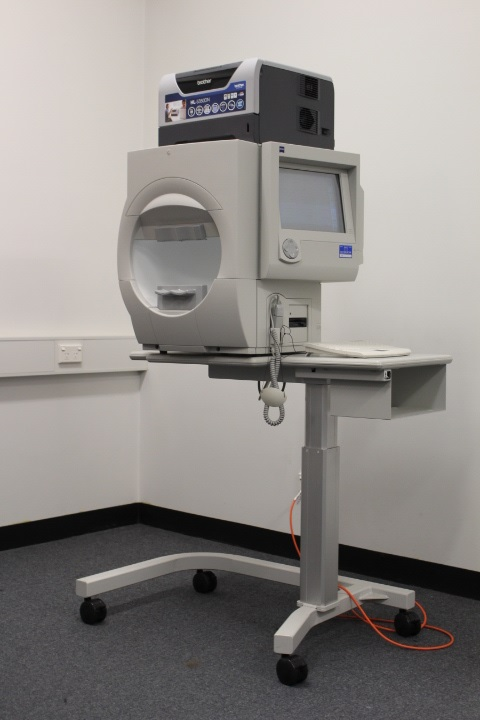
\includegraphics[width=0.5\textwidth]{hfa}
	\caption[\acl{HFA}]{\Iac{HFA} (``Humphrey VF'' by Sej licensed under \href{https://creativecommons.org/licenses/by-sa/4.0/deed.en}{CC BY-SA 4.0})}
	\label{fig:hfa}
\end{figure} 

\begin{figure}[p]
	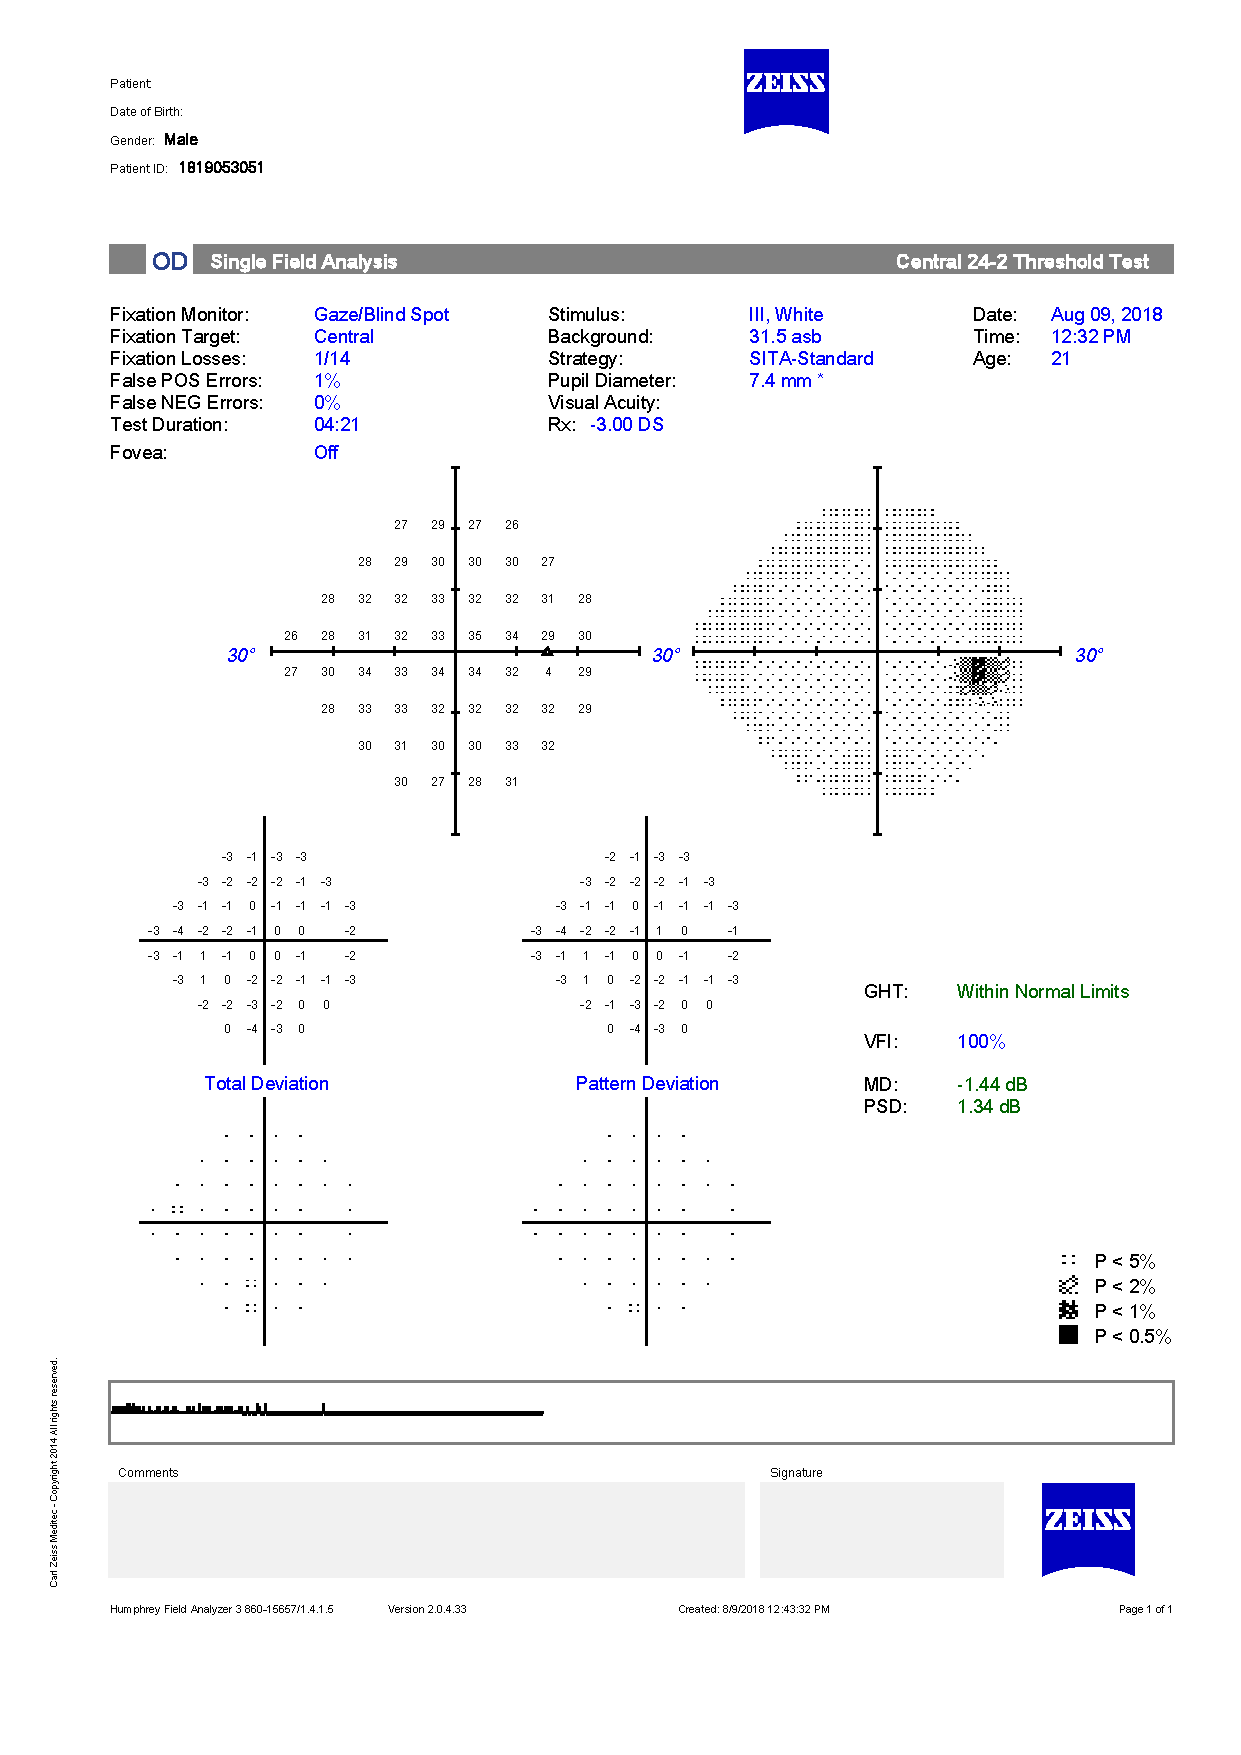
\includegraphics[width=0.9\textwidth]{report}
	\caption{Example of \iac{HFA} \acl{VF} test report}
	\label{fig:report}
\end{figure}

\begin{figure}[p]
	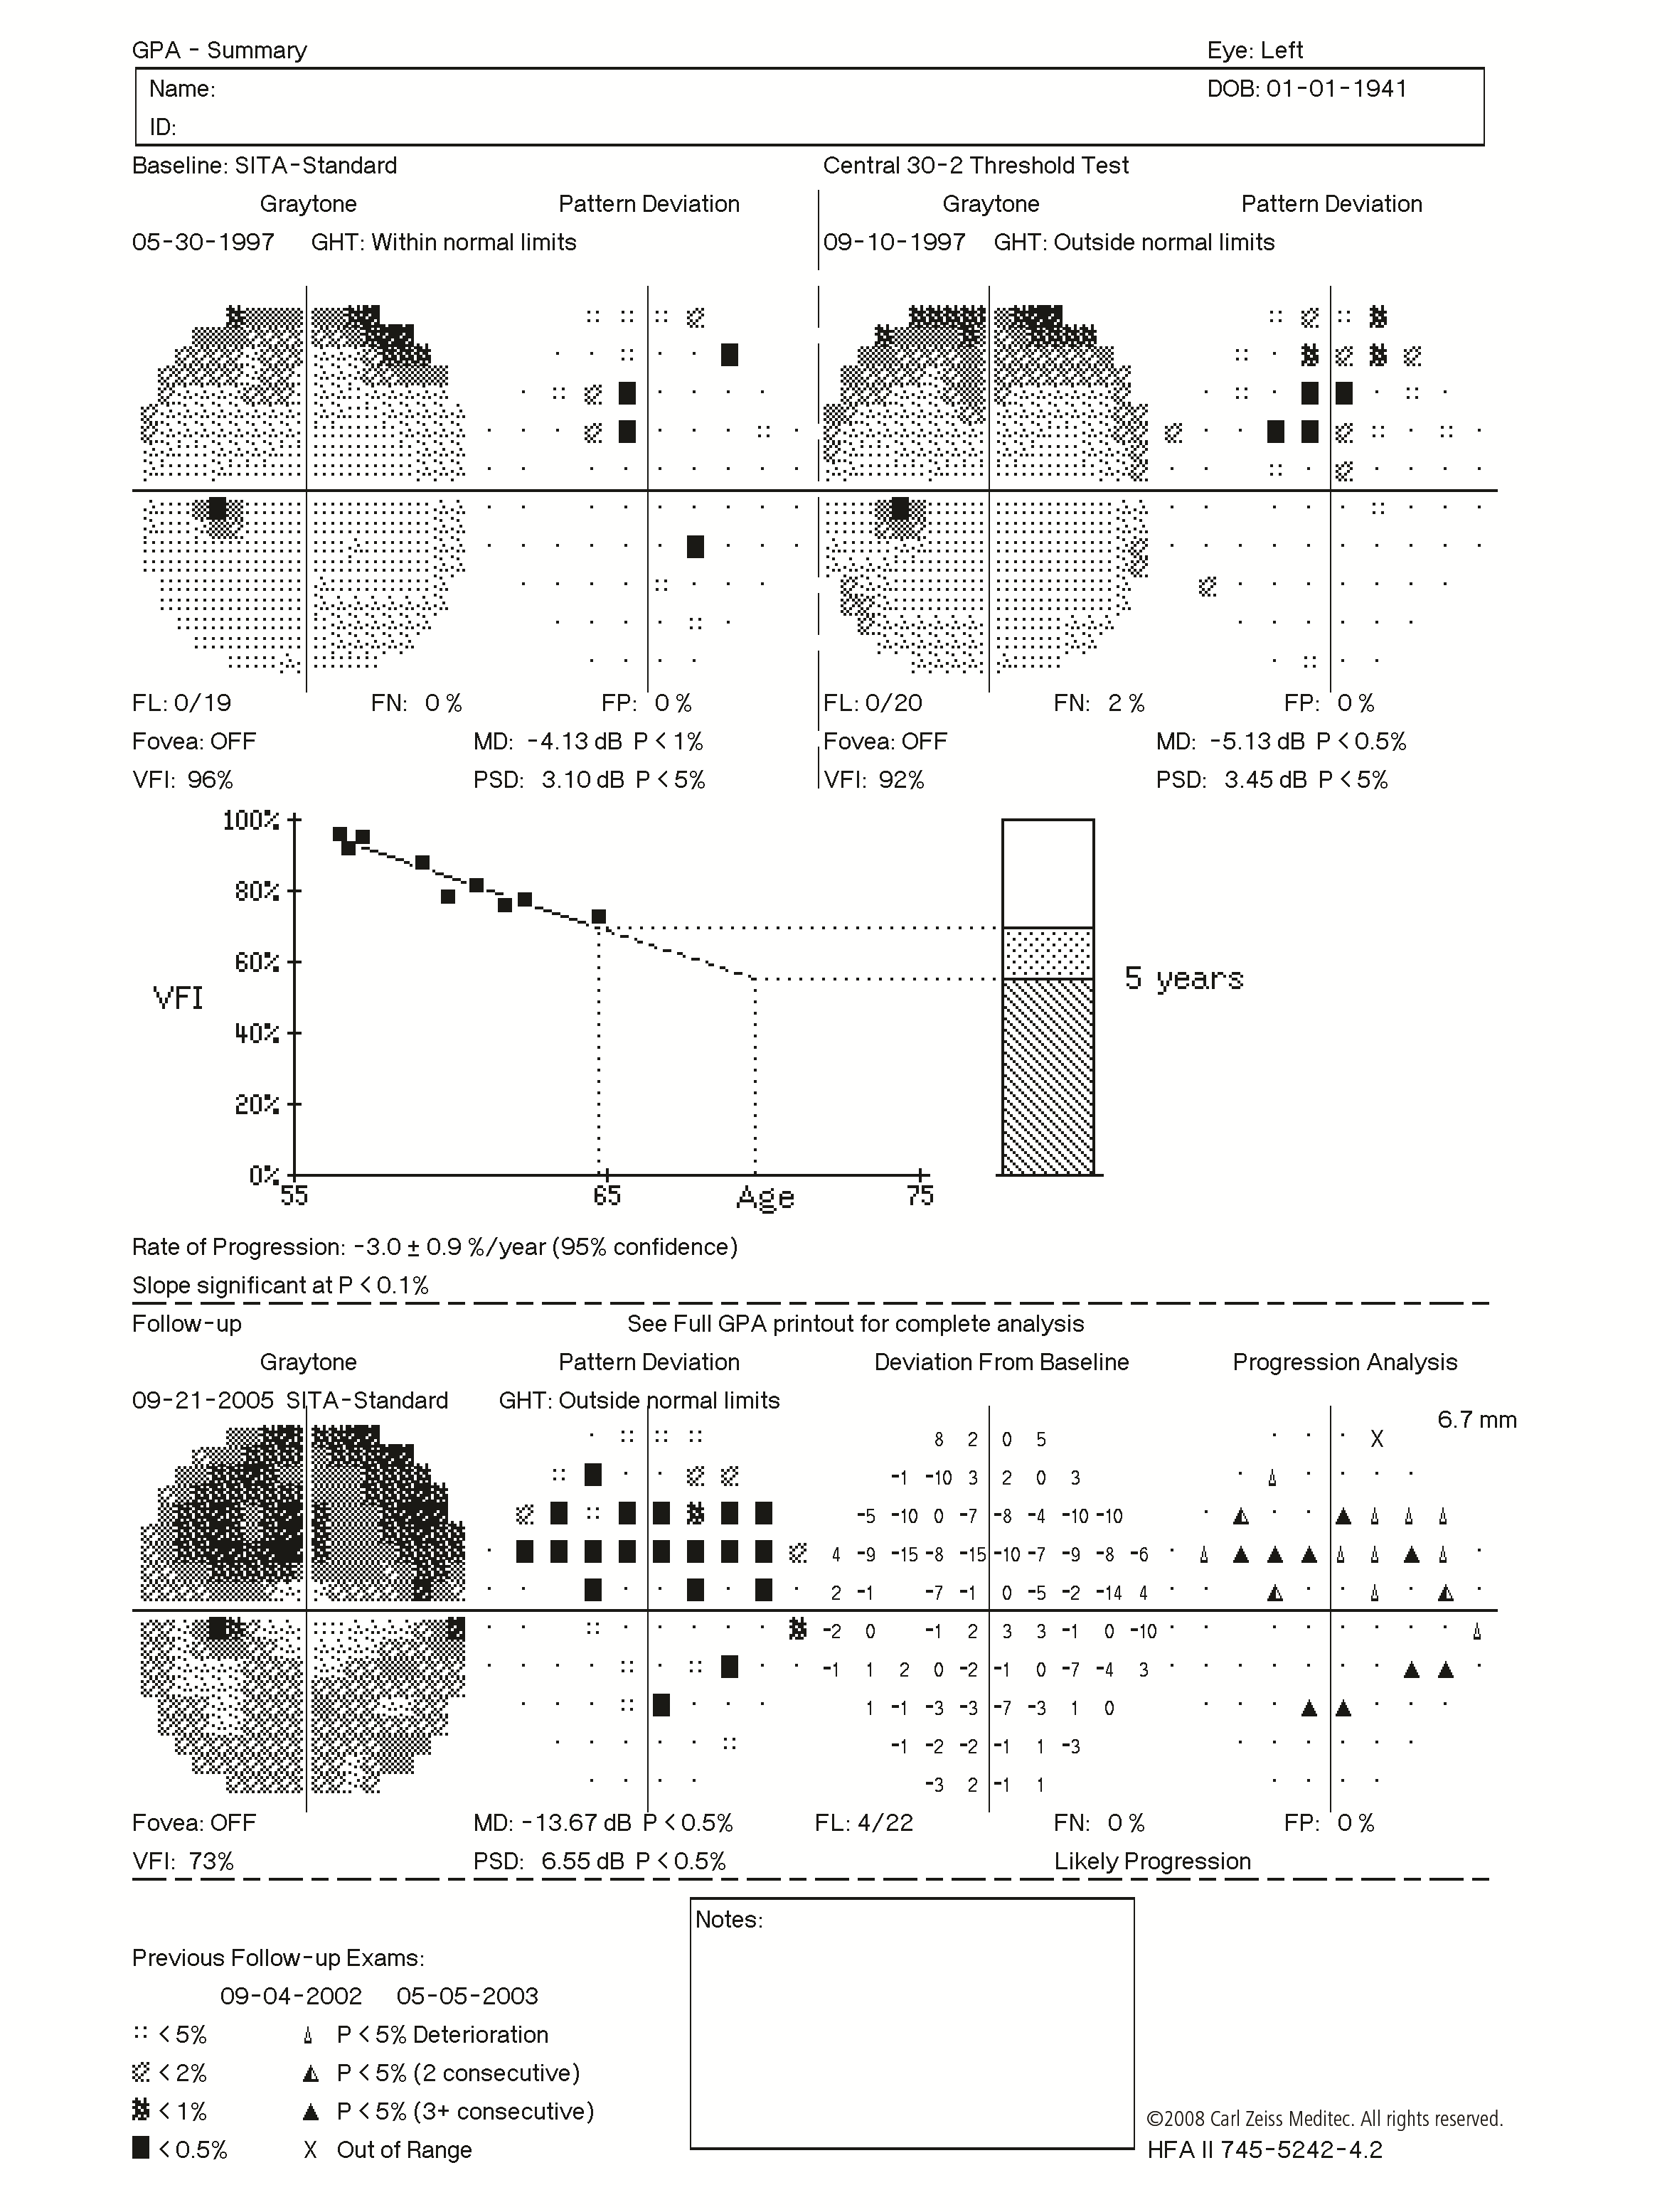
\includegraphics[width=\textwidth]{gpa}
	\caption[\Iac{HFA} progression analysis test report]{Example of \iac{HFA} progression analysis test report (Image from Carl Zeiss Meditec, Inc.)}
	\label{fig:gpa}
\end{figure}

\subsection{Single Field Analysis Metrics}

Historically Heijl et al. developed the two classic metrics for summarizing a \acl{VF}: \ac{MD} and \ac{PSD}. \cite{Heijl1987} First and foremost, to evaluate one's visual field, it is necessary to know the appropriate reference threshold ($N$) at each field location with an associated variance ($\sigma^2$). It is widely accepted that the human \ac{DLS} thresholds, in units of dB, can be modeled as a linear function of age. \cite{Heijl1987a} In general, the slope of loss of sensitivity is larger in mid-periphery than para-centrally, range from $0.5$ to $1$ dB/decade. The variance is also higher in mid-periphery than para-centrally. 

\ac{MD} is a measure of a \acl{VF}'s general mean value as compared to the reference. Mathematically, it is the mean of the difference between the measured threshold ($x$) and the reference $N$, weighted by the variance. Points with higher variance are considered less reliable and given less weight in the \ac{MD} metric; blind spots (i.e. ($15\degree$, $\pm3\degree$) are removed). MD values typically range from negative to slightly positive. Negative MD values indicate less than normal sensitivity in the entire \acl{VF} and the patient may be suspected of glaucoma and/or cataract.

\begin{equation} \label{eq:md}
\textrm{MD} =\frac{ 
\sum\limits_{i=1}^{n} \left\{
\frac{1}{\sigma_{i}^2} (x_i-N_i)
\right\} }{
\sum\limits_{i=1}^{n} 
\frac{1}{\sigma_{i}^2} 
}
\end{equation}

While the \ac{MD} is an intuitive summary metric for a \acl{VF}, it captures the general reduction in sensitivity, which is typical of cataract, but does not capture local asymmetries (variations) in the field, which is typical in a glaucomatous field. \ac{PSD} is another metric that tries to capture this asymmetry. Mathematically, it is defined as the weighted variance of the field, as defined in \cref{eq:psd}. $n$ refers to the numbers of locations, less the two blind spots, in the test pattern used for calculation (e.g. $n=54-2$ for the 24-2 pattern). \ac{PSD} is always positive, with higher value indicating a more varying field with a higher likelihood of glaucoma.

\begin{equation} \label{eq:psd}
\textrm{PSD}^2 =
	\frac{1}{n}
	\sum\limits_{i=1}^{n} 
	\sigma_{i}^2
	\times
	\frac{1}{n-1}
	\sum\limits_{i=1}^{n} 
	\frac{(x_i-N_i-\textrm{MD})^2}{\sigma_{i}^2} 
\end{equation}

Recently the new \ac{VFI} metric has become available on \ac{HFA} field analysis reports. It attempts to reduce the influence of cataract on \ac{MD} and is argued to be a better indicator for glaucoma doctors. It is reported as a percentage with $100\%$ being a perfectly healthy field and $0\%$ being a blind field. \cite{Bengtsson2008}

Another metric developed is \ac{GHT}. It combines measurement of the overall field sensitivity and differences between the top and half hemi-fields into a few hand-crafted ``if'' statements to report a field as one of the following categories for easy interpretation: \cite{Asman1992}

\begin{itemize}
	\item Abnormally high sensitivity
	\item Outside normal limits
	\item Borderline
	\item General reduction of sensitivity
	\item Within normal limits
\end{itemize}

These four metrics can be seen in figure \ref{fig:report}.

\subsection{Trend-Based Progression Analysis}

Currently, the main approach to determine glaucoma progression is a trend-based analysis by performing \ac{OLSLR} on MD. The \ac{HFA} Guided Progression Analysis reports \ac{OLSLR} on its \ac{VFI} that offers similar information. The fitted trend is typically extended five years into the future, and the slope of the line is used to classify patients into three categories (mild: $0$ to $-0.4$ dB/year, moderate: $-0.5$ to $-2$ dB/year, and severe: $<-2$ dB/year). \cite{Chauhan2008} Glaucoma specialists combine these data with additional information such as the thickness of the retinal fiber layer in the macula, \ac{IOP} and the cup-to-disk ratio to determine the optimal plan of treatment. 

\subsection{Limitations}

The current method of evaluating \acl{VF} information is limited in its robustness. For example, \ac{VFI} may remain at $100\%$ in $22\%$ patients who have MD of $-5$ dB or better. Hence early progression (up to $-5$ dB) may be missed if VFI alone is used. Moreover, based on a semi-annual follow-up schedule, at least five fields are required to produce an accurate prediction for a disease that is progressing at moderate rates (the slope of the OLSLR on MD is $-1.0$ dB/year). \cite{Chauhan2008} This means that meaningful decision about the progression of the disease cannot be made until at least two years after the initial visit. 

Last but not least, \ac{OLSLR} is a simple model chosen based on its mathematical simplicity but not upon physiology. Since glaucoma can be caused by multiple neurological pathways, it is argued that the progression trend is likely nonlinear in nature. \cite{Pathak2013} 

In short, the use of linear regression to predict \acl{VF} loss and the need for a long observation period impede timely and accurate decision making by the clinician. A better method that can provide more accurate information to the clinician in fewer \acl{VF} tests can allow more effective intervention for glaucoma patients in the disease's early stages. This is the primary motivation for the alternative models reviewed below and for the current work.

\section{Literature Review: Alternative Progression Models}

This section will review alternatives to the \ac{OLSLR} on MD model for \acl{VF} progression prediction. 

\subsection{Statistical Models}

A complement to trend-based analysis is event-based analysis. A popular implementation is the Glaucoma Progression Analysis (GPA) since it is provided by the \ac{HFA}. Instead of fitting a trend on a global index, the progression of each point in the field with respect to a baseline measurement is considered. On average, this method is found to have low false-positive rate. However, this is dependent upon achieving a good baseline and does not work for patients with severe \acl{VF} loss. \cite{Aref2017}

Other non-linear models suggest fitting an exponential model to the \acl{VF} indices. For example, Pathak et al. argued that an exponential model is better supported by recent knowledge of structure-function relationship than a linear model. \cite{Pathak2013} They demonstrated that a linear mixed-effect (LME) approach with an exponential model provided significantly better prediction of glaucoma progression than linear models. However, it is also pointed out that even though the LME approach has better results than the \ac{OLSLR} it still cannot capture the full extent of glaucomatous \acl{VF} change.

Other innovative approaches to the glaucoma progression problem in the literature include:

\begin{itemize}
	\item Point-wise linear regression (PLR): Developed for improving early detection, PLR combines event-based and trend-based analysis \cite{Nouri-Mahdavi2005}. 
	\item Analysis with Non-Stationary Weibull Error Regression and Spatial Enhancement (ANSWERS): Using spatial correlation between points and incorporating non-stationary variability; progression detection was found to be better especially in short time series \cite{Zhu2015}.
	\item Spatially filtering \acl{VF} data before PLR analysis: By applying a spatial filter that incorporates physiological relationships between measured contrast sensitivities at test points within the visual field, the specificity of the PLR method is not affected but the sensitivity of detecting the rate of progression is improved \cite{Strouthidis}.
\end{itemize}

\subsection{Machine Learning Models}

The above methods use different approaches to improve the prediction of glaucoma progression and demonstrate the complexity of the prediction task. This is not surprising due to the complex nature of the disease. A natural step forward involves leveraging the power of modern \ac{ML} techniques to integrate features such as non-linear trends, correlation between \acl{VF} test locations, field patterns, etc. into a single model.
 
Existing studies have demonstrated the usefulness of \ac{ML} in glaucoma care. For example, Asaoka et al. compared the performance of traditional ML classifiers with that of a deep feed-forward neural network (FNN) in diagnosing preperimetric glaucoma with visual field data \cite{Asaoka2016}. Their FNN model performed significantly better than other methods. In another study, Yousefi et al. applied clustering algorithms to extract visual field patterns as features, then adapted the traditional linear regression algorithm to model the features to generate the predictions \cite{Yousefi2018}. The \ac{ML}-based index for the detection of glaucoma progression outperformed current methods. 

However, these studies either did not directly address the problem of predicting \acl{VF} progression or only used traditional \ac{ML} methods for initial feature extraction. In a recent study that fully utilized the power of \ac{ML} for the prediction task, Wen et al. \cite{Wen2018} used deep learning network to predict future visual field given the measurements of a single current \acl{VF}. Their deep learning network demonstrated amazing capability to generate prediction for future visual fields for up to $5.5$ years with a correlation of $0.92$ between the predicted \ac{MD} and actual future \ac{MD} (average difference of $0.41$ dB). Their results suggest the tremendous potential of this research area. 

Another benefit of using an \ac{ML} model is the ability to use visual field data (i.e. functional indication of \acl{VF} integrity) and \ac{OCT} data (i.e. structural indication for the integrity of the retina) at the same time. It is known that by utilizing both \acl{VF} and \ac{OCT} data the sensitivity of glaucoma detection can be improved \cite{Shah2006}, \cite{Lu2008}. Multivariate models including both \acl{VF} and \ac{OCT} have also been shown to be successful \cite{Mwanza2013}. However, there is limited research on combining \acl{VF} and \ac{OCT} features through a \ac{ML} model. A limited attempt to explore this idea by Silva et al. did not produce better results than those obtained by \acl{VF} only parameters \cite{Silva2013}. 

In our study we plan to use \ac{ML} models that combine \acl{VF} and \ac{OCT} data for prediction of disease progression.  Specifically, we will use a deep \ac{RL} approach to the glaucoma progression problem. Deep RL has gained attention lately due to its use in solving seemingly impossible problems. The most well-known example is solving the ancient Go game, which is considered to be orders of magnitude more difficult than chess and other board games \cite{Silver2016}. \ac{RL} has also been used in the context of healthcare for discovering optimal, individualized treatment strategies for lung cancer \cite{Zhao2009}\cite{Zhao2011}, HIV \cite{Ernst2006} and neurological disorders \cite{Shortreed2011}. To the best of our knowledge this will be the first study to use \ac{RL} to predict glaucoma progression. 



\chapter{Progress to Date}

\section{Rotterdam Longitudinal Glaucomatous \ac{VF} Dataset}

The Longitudinal Glaucomatous Visual Field data from Rotterdam Ophthalmic Data Repository \cite{Bryan2013} consists of data from $139$ patients' $278$ eyes. A total of $4863$ 24-2 test results with MD are available. On average each eye has $17.5$ fields available with mean follow-up time of $9.2$ years. $270$ $(97.1\%)$ eyes have at least $14$ fields with a minimum of $7.6$ years of follow-up. The mean and median follow-up interval between tests is $203$ and $189$ days; the standard deviation of follow-up time is $72.3$ days. $346$ $(7.5\%)$ of follow-ups had an interval of more than $270$ days. 

\subsection{Data Characteristics}

To investigate the composition of healthy versus glaucomatous patients the dataset, the characteristic of MD values in the dataset is investigated. In figure \ref{fig:mean_md_hist} the distribution of average MD value calculated from all tests administers on an eye for each of the $278$ eyes is shown. The mean and median of the distribution are $-8.9$ and $-6.8$ dB respectively. The data set contains mostly eyes with mild to moderate reduced MD values ($75\%$ of eyes have average MD $>-13.2$ dB).

\begin{figure}[h]
	\centering
	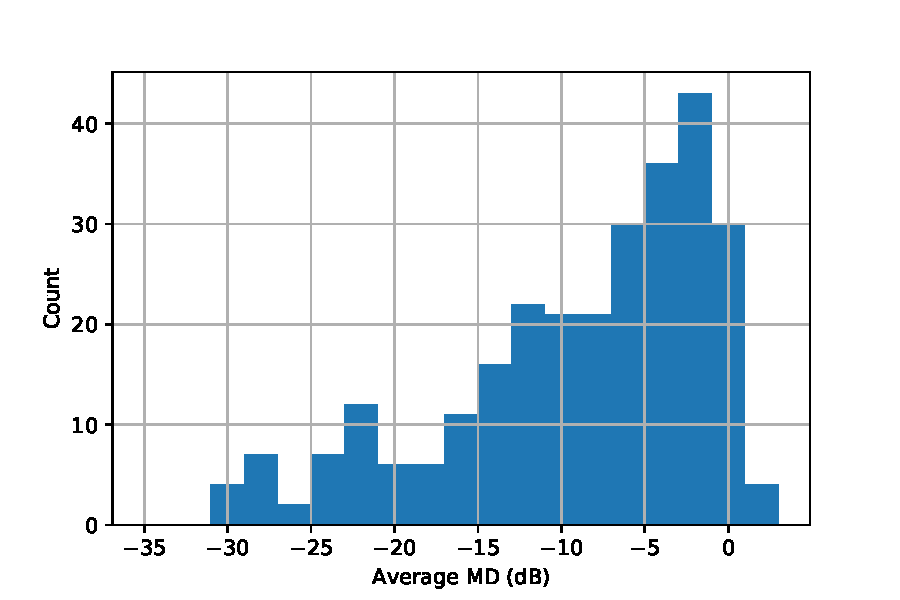
\includegraphics[width=0.6\textwidth]{mean_md_hist}	\caption{Distribution of eyes' average MD values within the Rotterdam dataset ($n=278$)}
	\label{fig:mean_md_hist}
\end{figure}
%
%\begin{figure}[h]
%	\centering
%	\begin{subfigure}[b]{0.45\textwidth}
%		\centering
%		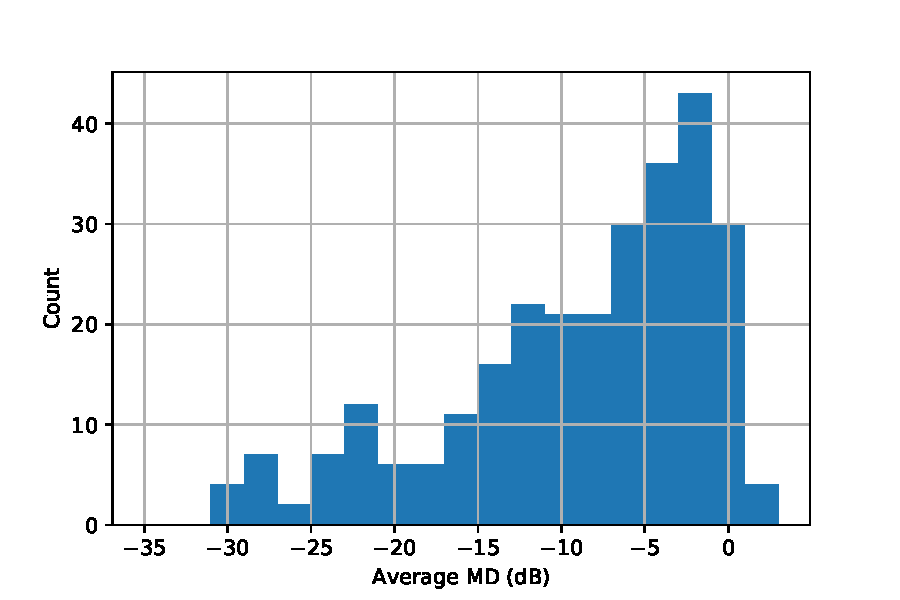
\includegraphics[width=\textwidth]{mean_md_hist}
%		\caption{}
%		\label{fig:mean_md_hist}
%	\end{subfigure}
%	\hfill
%	\begin{subfigure}[b]{0.45\textwidth}
%		\centering
%		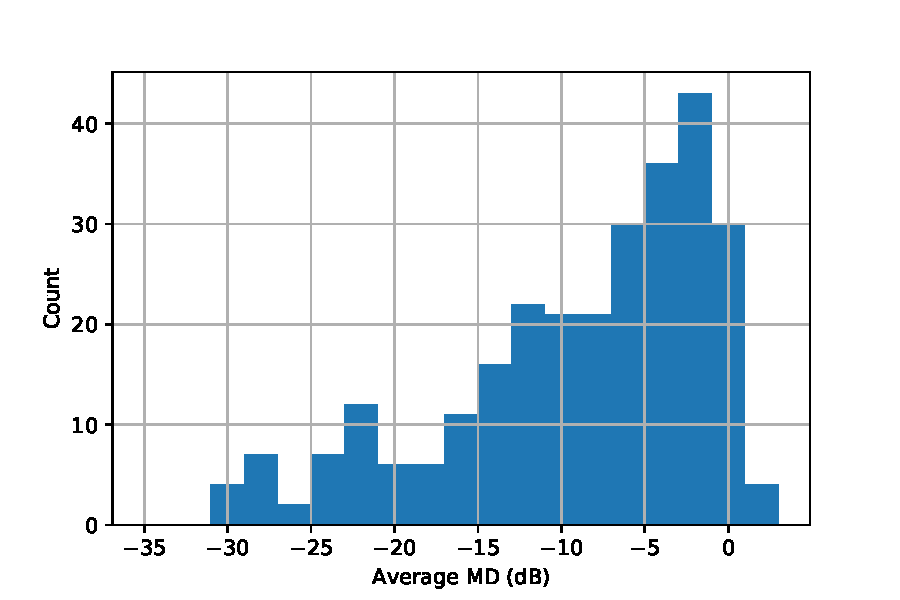
\includegraphics[width=\textwidth]{mean_md_hist}
%		\caption{}
%		\label{fig:three sin x}
%	\end{subfigure}
%	\caption{(a) Distribution of MD values within the patient dataset}
%	\label{fig:study_site}
%\end{figure}
%
%
%
%


\chapter{Future Work}

\section{Data collection}

\begin{itemize}
	\item Already performed: obtain REB approval for retrospective data collection
	\item Already performed: design data collection procedure, including data collection form, anonymization and parsing program
	\item Late January: meeting with Toronto Western Hospital research and clinical staff to initialize data collection process
	\item Early February: finalize data collection procedure and start mass data collection
	\item Late February: preliminary database establish at similar size scale of the Rotterdam dataset
	\item March to future: continued data collection
\end{itemize}

\section{Literature Algorithm Implementation}

\begin{itemize}
	\item February to March: Implement algorithms in literature for comparison against our approach
\end{itemize}

\section{Deep Learning Algorithm Design}

\begin{itemize}
	\item Current: A preliminary deep neural network design is in place, consisting of \iac{CNN} for spatial feature detection and \iac{LSTM} \ac{RNN} for temporal sequence feature detection. The features are concatenated and passed to a fully connected network for final output. 
	
	\begin{figure}[h]
		\centering
		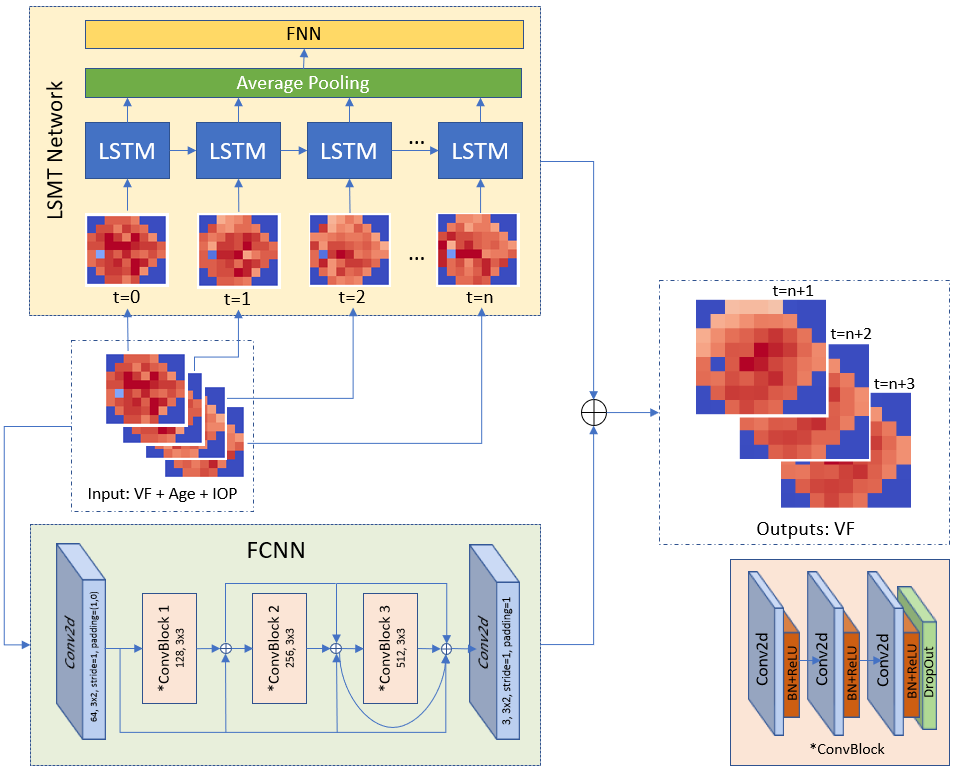
\includegraphics[width=\textwidth]{nn_struct}	\caption{Proposed neural network structure}
		\label{fig:nn_struct}
	\end{figure}

	\item February: Fix current issues present in the algorithm implementation and evaluate network performance against other methods.
	
	\item March: Preliminary testing of designed network on the collected Toronto dataset.
	
\end{itemize}



%% This adds a line for the Bibliography in the Table of Contents.
\addcontentsline{toc}{chapter}{Bibliography}
%% *** Set the bibliography style. ***
%% (change according to your preference/requirements)
\bibliographystyle{IEEEtran}
%% *** Set the bibliography file. ***
%% ("thesis.bib" by default; change as needed)
\bibliography{thesis}

%% *** NOTE ***
%% If you don't use bibliography files, comment out the previous line
%% and use \begin{thebibliography}...\end{thebibliography}.  (In that
%% case, you should probably put the bibliography in a separate file and
%% `\include' or `\input' it here).

\end{document}
